\section{Behavioral Patterns}
\fxnote{Skriv intro}

\subsection{Food Class}

Added -> Expired -> Quantity changed -> Removed
Added -> Quantity changed -> Expired -> Quantity changed -> Unexpired -> Removed
Shopping list item added -> Added -> Expired -> Removed
Shopping list item added -> Shopping list item removed

\begin{figure}[tbhp]
	\centering
	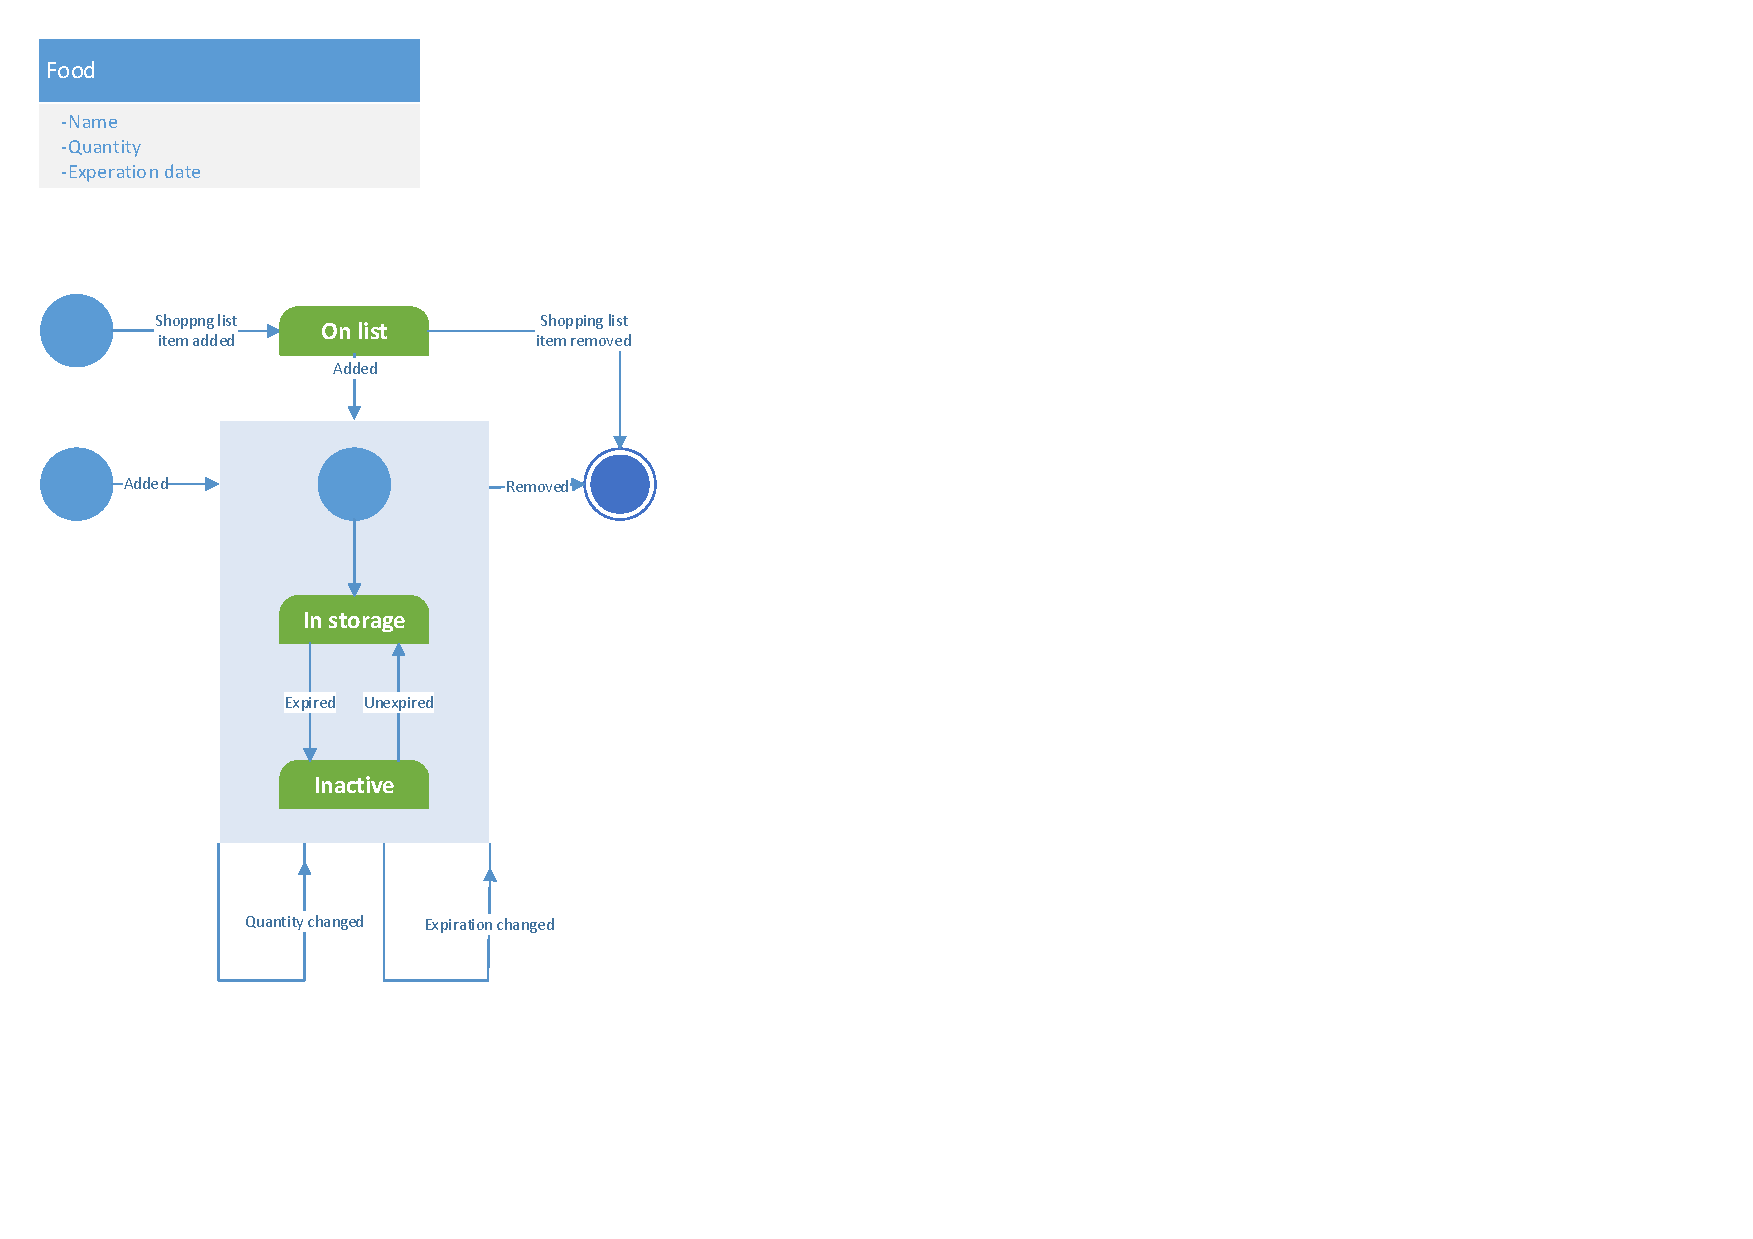
\includegraphics[clip=true, trim=0.5cm 4cm 18.5cm 0.5cm,  ]{Development/ProblemDomain/FoodClass.pdf}
	\caption{Behavior diagram for the food class} \label{FoodClass}
\end{figure}
The \textbf{Food} class contains information about the quantity and expiration date of a food item. The food items can be found in the lists inventory or shopping list.

\subsection{Meal Class}

Meal added -> Change scale -> Meal prepared
Meal added -> Change date -> Meal prepared
Meal added -> Day passed -> Reschedule meal -> Meal prepared
Meal added -> Change scale -> Change date -> Change scale -> Meal prepared

\begin{figure}[H]
	\centering
	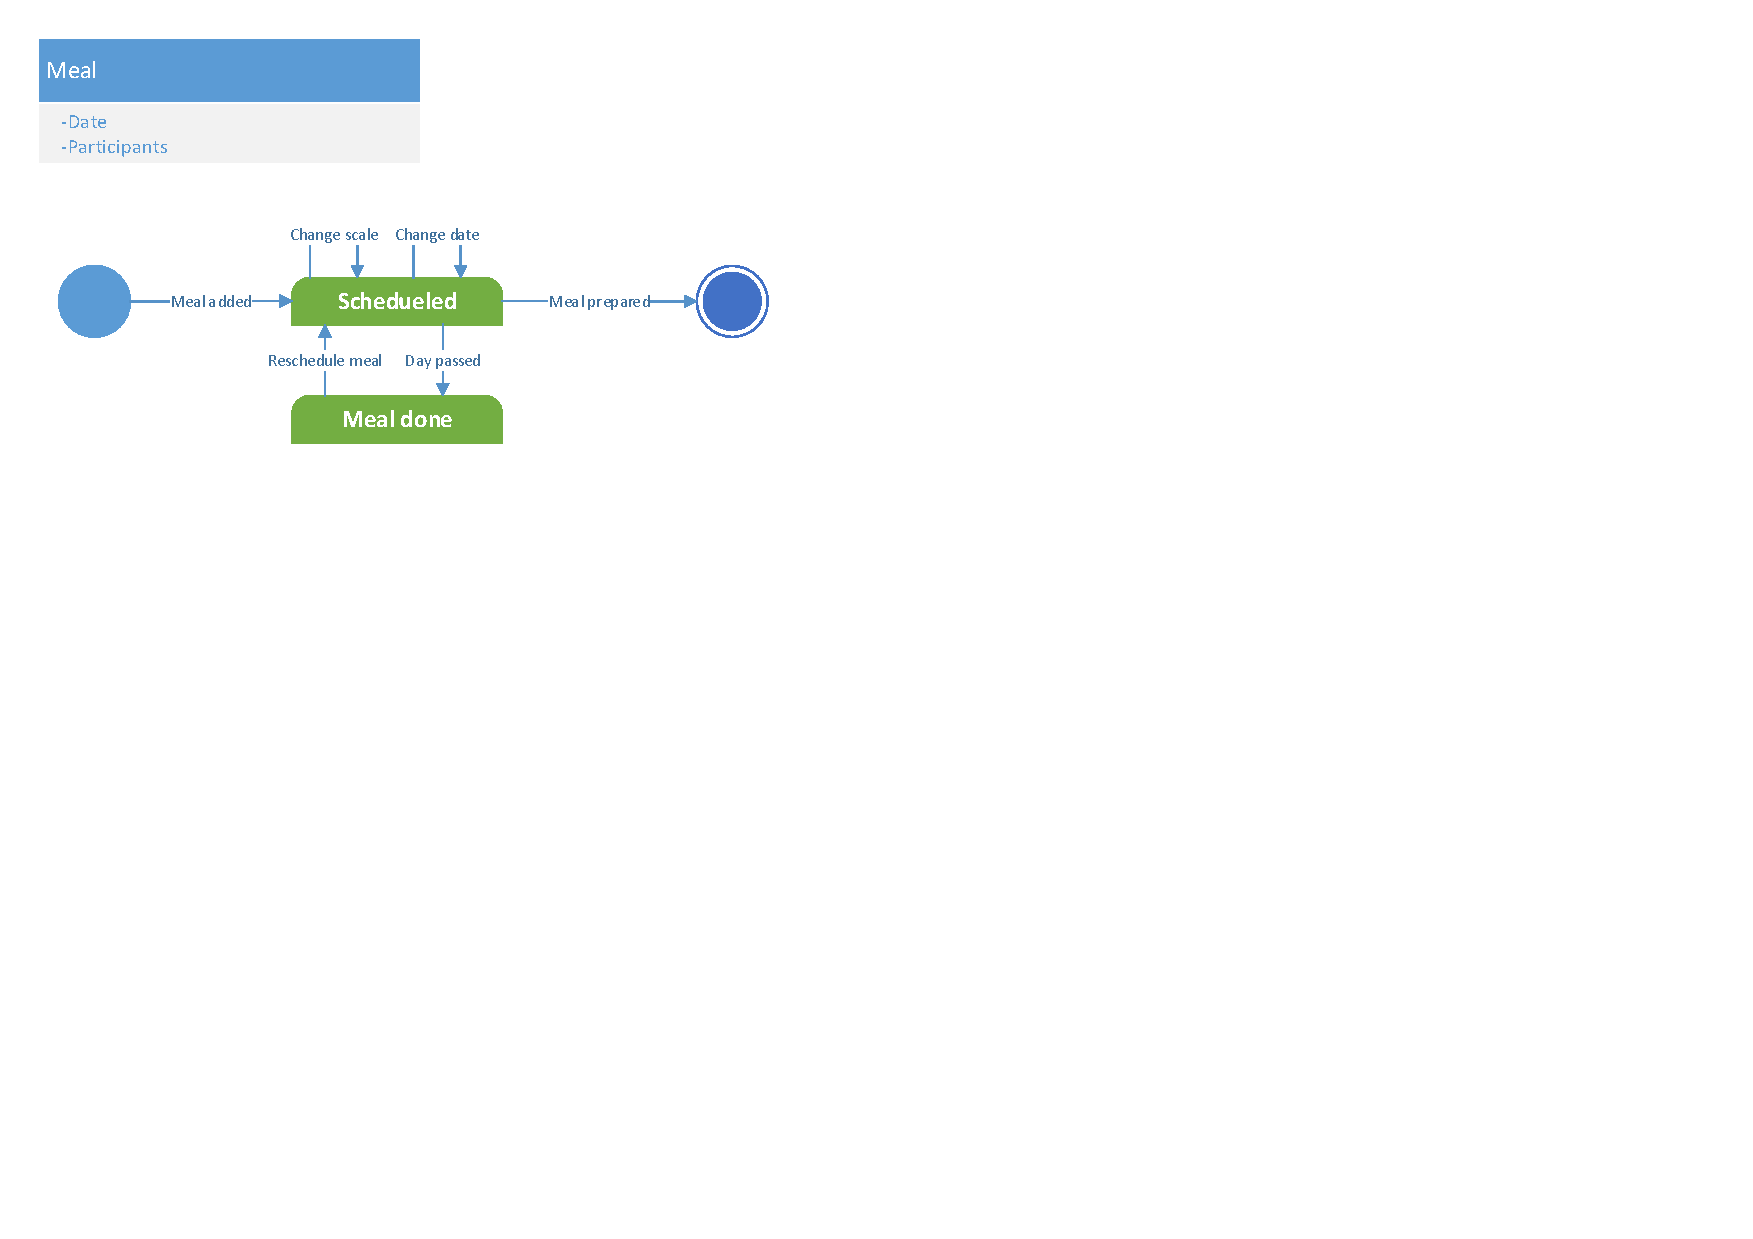
\includegraphics[clip=true, trim=0.5cm 13cm 16.5cm 0.5cm]{Development/ProblemDomain/MealClass.pdf}
	\caption{Class diagram for the meal class} \label{MealClass}
\end{figure}
The \textbf{Meal} class contains information about a meal and when to make it. It consists of recipes.

\subsection{User Settings Class}

\fxnote{Anders: Start and finish for the diagram is needed}

\begin{figure}[H]
	\centering
	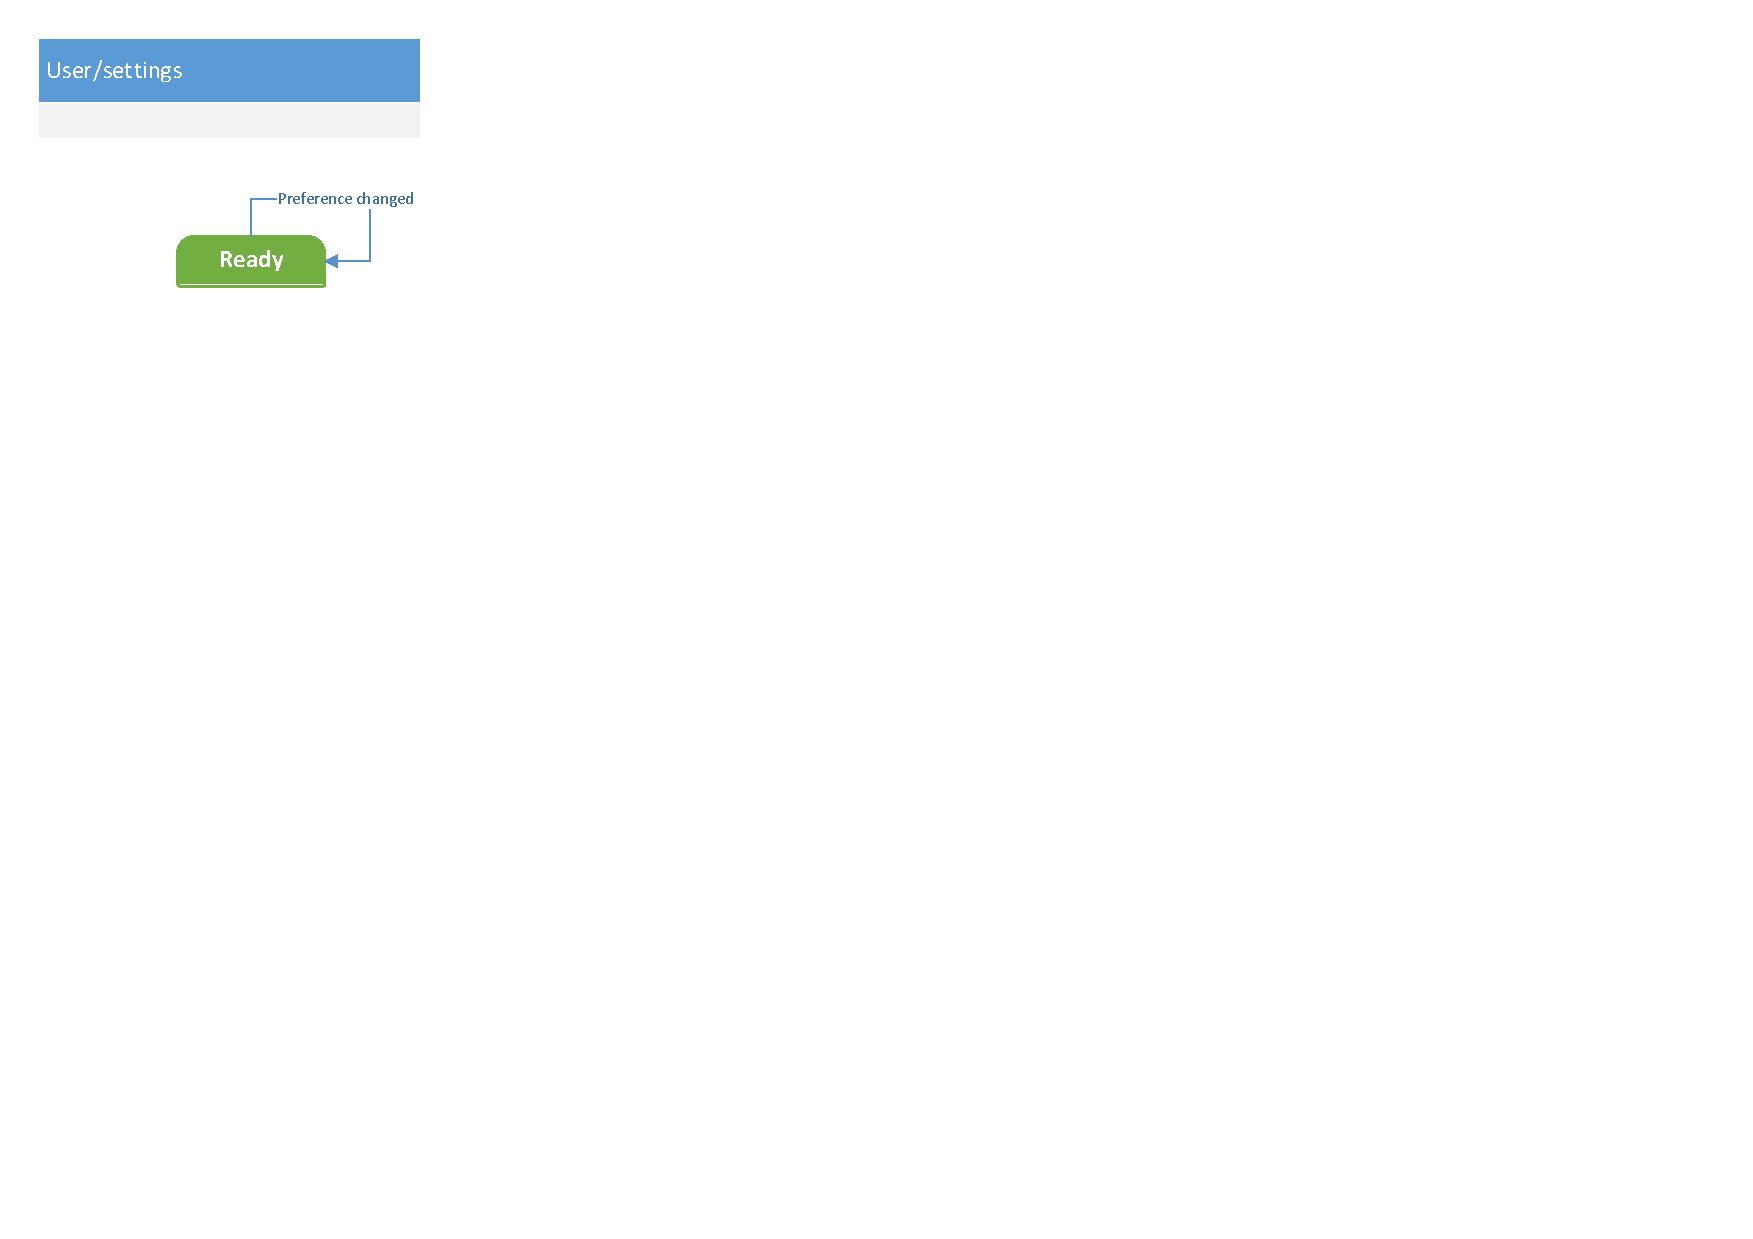
\includegraphics[clip=true, trim=0.5cm 15.5cm 22.5cm 0.5cm]{Development/ProblemDomain/UserSettingsClass.pdf}
	\caption{Class diagram for the user settings class} \label{UserSettingsClass}
\end{figure}
The \textbf{User settings} class contains preferences from the user which the system should take into consideration.

\subsection{Recipe Class}

Recipe added -> Recipe removed
Recipe added -> Recipe found -> Meal added -> Meal Removed
Recipe added -> Recipe found -> Recipe found -> Meal added -> Meal Removed

\begin{figure}[H]
	\centering
	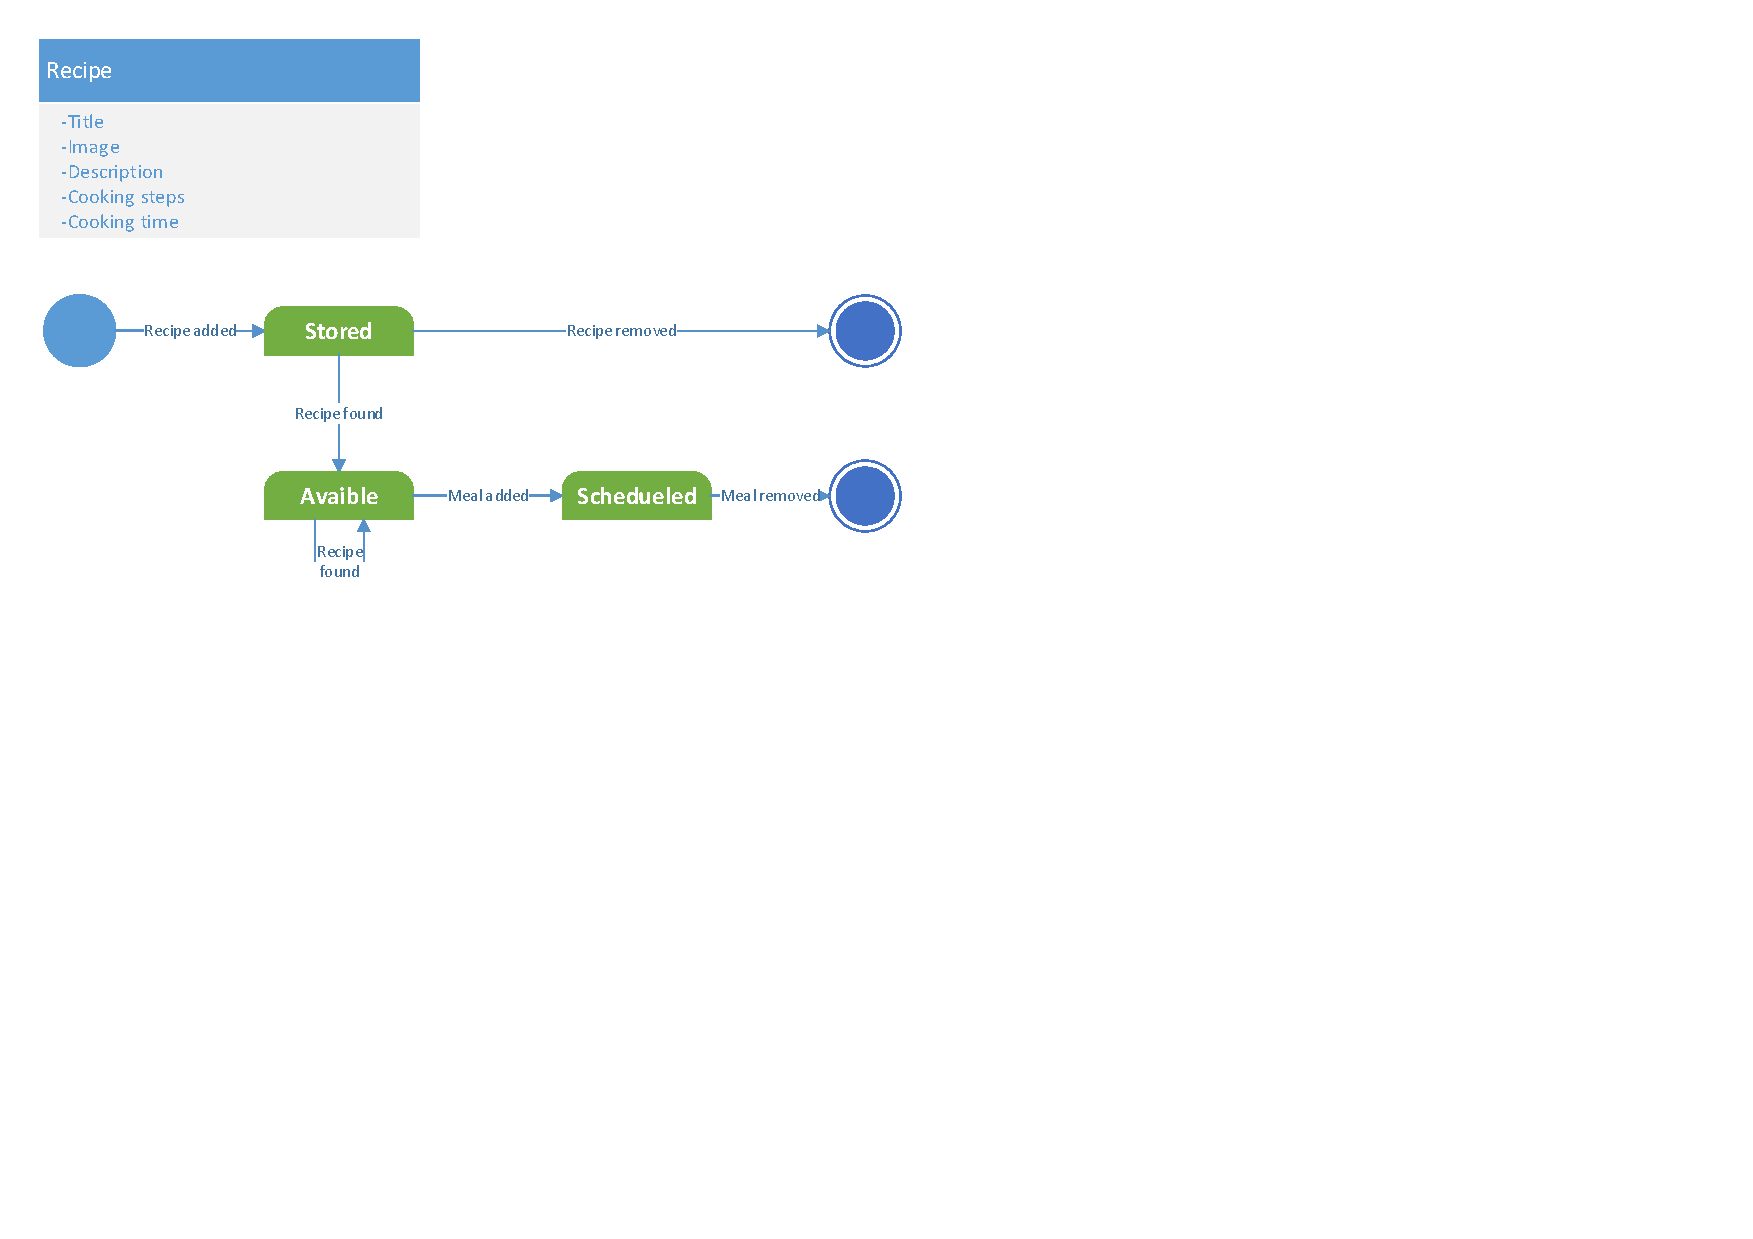
\includegraphics[clip=true, trim=0.5cm 11cm 14cm 0.5cm]{Development/ProblemDomain/RecipeClass.pdf}
	\caption{Class diagram for the recipe class} \label{RecipeClass}
	\end{figure}
\textbf{Recipes} consists of \textbf{Food}. It also contains information on how to prepare the meal from the recipe.